\documentclass[10pt,conference,compsocconf]{IEEEtran}

\usepackage[utf8]{inputenc} % For characters diacritic symbols
\usepackage{hyperref}
\usepackage{graphicx}	% For figure environment

\begin{document}

\title{Machine Learning Course - Class Project 1}

\author{
  Hrvoje Bušić, Dino Mujkić, Sebastijan Stevanović\\
  \textit{EPFL Lausanne, Switzerland}
}

\maketitle

\begin{abstract}
Examining and categorizing decay signatures of proton collision events is a crucial part in indirect observation of Higgs' boson. With four different implementations for the linear regression function and two additional for the logistic regression, this project evaluated the efficacy of the different models with the aim to categorize signatures to those that belong to Higgs' boson (signal) and those that belong to other particles (background). Furthermore, with the aim of obtaining better results utilizing the aforementioned models, extensive data processing and feature selection was applied to the provided training set.
\end{abstract}

\section{Introduction}

The Higgs boson is an elementary particle in the Standard Model of physics, which explains why other particles have mass. Protons during a collision at high speeds generate smaller particles as by-products of the collision, and rarely these collisions can produce a Higgs boson. As Higgs boson decays rapidly into other particles, scientists don't observe it directly, but rather measure its decay signature. 

Many decay signatures look similar, and in this project we used different machine learning algorithms to train models for predicting whether the given event's signature was the result of a Higgs boson (signal) or some other process/particle (background).

Important part in the training of the models is the preprocessing and feature selection from the data set. Separation of entries by relevant features proved crucial in training models that perform with a high level of accuracy in the validation phase.

\section{Data processing and model evaluation}

Our initial approach was to simply evaluate how well the different models performed on the raw data set to get a preliminary picture of the accuracy for each model. Having only a limited number of daily submission attempts, we opted to perform this testing by splitting the data set into a training and validation set with a ratio of 70\% to 30\% respectively. This method of evaluating different models proved to be rather effective since the changing values of mean square error (MSE) we would obtain for our validation sets would reflect quite well the changing scores we would obtain on Kaggle. Thus, this method of testing was used throughout our data processing and model evaluation to predict the accuracy of the model (weights).

Following this initial testing with limited results, we decided to focus on processing our data set since it was evident that there are many missing values. Firstly, we wanted to find a way to deal with these missing/invalid values (values of -999). Our initial approach was to remove all columns that have more invalid values than valid with the assumption that these columns would not be effective for improving the model since they lack so much information. Additionally, for the remaining columns that contained invalid values, we calculated the mean for each column and replaced the invalid values with their corresponding column mean. This was done under the assumption that inserting the mean value would not affect negatively the accuracy of the model and thus were better than the invalid values. All the data was then normalized, and the mean and standard deviation were saved so that we can reuse the same for the test set.

Having the goal to also improve our previous simple models and taking into account that we have deleted quite a few columns previously, we decided to also test whether a polynomial basis approach would yield a better result. To do this, we tested different degrees for the polynomial basis and indeed noticed the possibility to improve our model in this manner. Our validation RMSE would decrease up until degree 7, following which it would start quickly increasing (likely due to over-fitting), and thus we opted for a polynomial basis of degree 7. Now, the accuracy score we got on Kaggle for this approach, combining data preprocessing with a polynomial basis of degree 7, was 0.78489.

\begin{figure}[h]
  \centering
  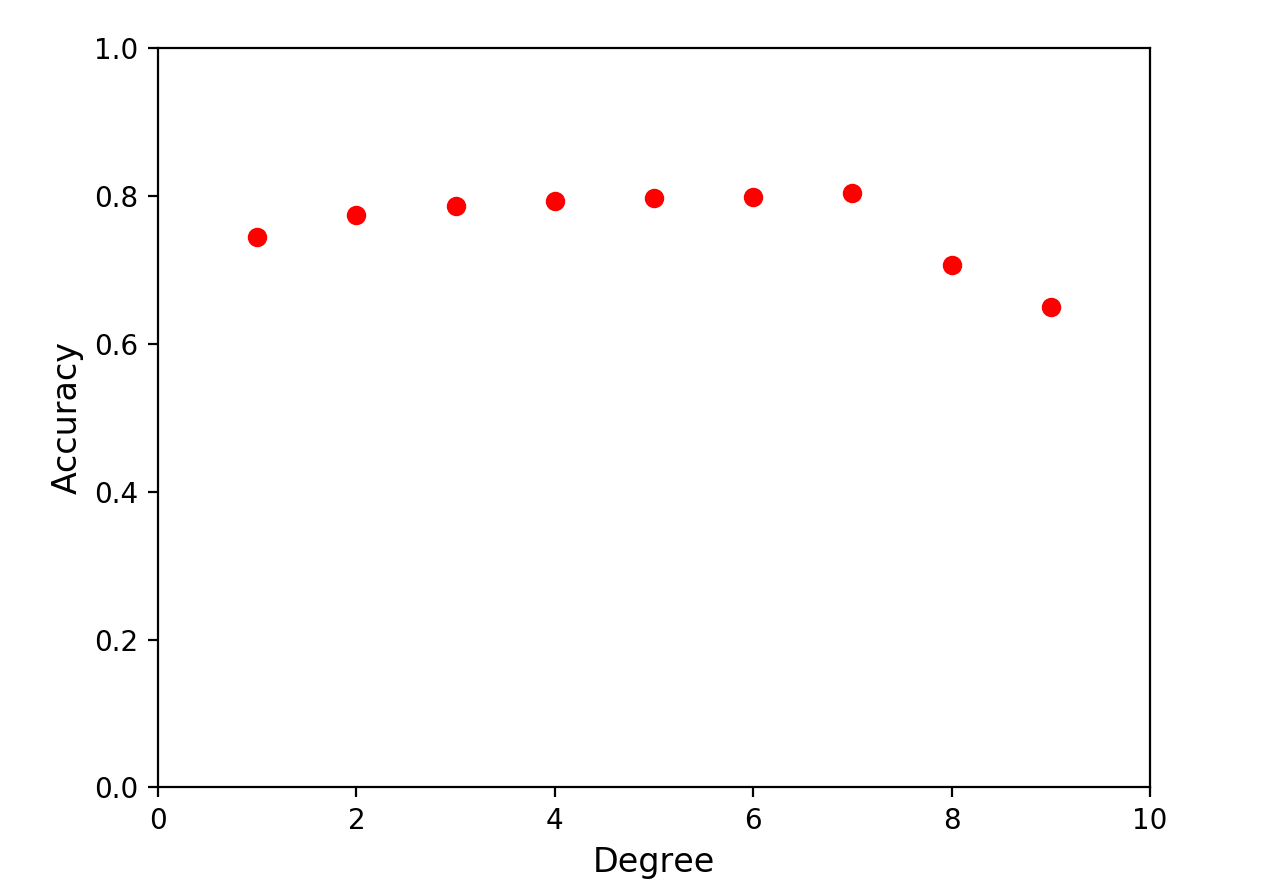
\includegraphics[width=\columnwidth]{polynomial_basis_degrees}
  \caption{Accuracy for different polynomial basis degrees.}
  \vspace{-3mm}
\end{figure}

This was quite an improvement, but we then decided to test whether our previous assumptions regarding data cleaning were correct. We then found out that without deleting columns that have more invalid values and just by replacing the invalid values with their corresponding column mean, we get a better score, 0.79443. Additionally, we considered whether we should use a median instead of a mean since the median is more resistant to outliers. However, this led to only a slight improvement of our score.

Following these approaches, we decided to look more closely into the values of each column. Since we observed that the column 'PRI\_jet\_num' was quite different from others, we decided to test whether eliminating it would lead to an improvement. Surprisingly and strangely, deleting this column got us the best score thus far, 0.80468. However, all of our previous assumptions were made without a true in-depth analysis of the data set and thus we decided to perform exploratory data analysis about our previous result and how to achieve an even better result. We started from our 'strange' column 'PRI\_jet\_num'. It appeared that the only possible values for this column were in the range from 0 to 3 (inclusive). We also noticed that the other columns depend quite highly on this column, especially in the terms of missing values. Hence, we then decided to split our data set into four data sets based on 'PRI\_jet\_num' value and this led to our biggest breakthrough. All the invalid values were now grouped in certain columns for each of the data sets. Thus, we just had to delete all the columns that have all the invalid values within each of our 4 data sets. After that, the only column that had invalid values was 'DER\_mass\_MMC'. Hence, we decided to split our data sets into ones that have invalid values and ones that do not have. In the end, we ended up with 8 different sets. Furthermore, we deleted a few more columns that we discovered were irrelevant or redundant through correlation testing and analysis. For example, for our set with 'PRI\_jet\_num' = 0, we deleted also the column 'DER\_pt\_h' because 'DER\_pt\_h' is always equal to 'DER\_pt\_tot'. Understandably, all the data wrangling which we perform on the train set, was also done on test set, so we end up with 8 train sets and their 8 respective test sets. With this approach, we also had to take in account data ids due to the data splitting with which we would end up with 8 arrays of predictions with shuffled data. To fix this, we had to join the predictions into one array and sort them by the id.

\section{Final method}

Following this improved data and feature processing, we noticed a significant improvement in our accuracy. Furthermore, we now observed that we get different results for different polynomial basis degrees for each of the training sets. Thus, through the process of cross validation with selection of different degrees, we discovered the optimal degree for the polynomial basis for each of the training sets. Thus, using the preprocessed and cleaned data sets with their respective polynomial basis degrees, we obtained our best results by applying the least squares method with the final accuracy score of 0.82728.

\section{Summary}

The aim of our project was to build a highly accurate machine learning model for categorizing proton collision events. We explored four different implementations of the linear regression algorithm and two additional algorithms for the logistic regression. Research included thorough preprocessing of the given data set and appropriate feature selection. While we were able to train a model with a high level of accuracy on the final test set (0.82728), consideration of other machine learning models such as neural networks with appropriate tuning offers new approaches to obtain results of even higher accuracy.

\end{document}